\documentclass{article}
\usepackage[utf8]{inputenc}
\usepackage{graphicx}
\usepackage{float}
\usepackage[francais]{babel}
\usepackage[T1]{fontenc}
\title{Rapport du Projet de Programmation en C}
\author{Kaïs-Khan Hadi et Raphaël Gilliot}
\date{Décembre 2018}

\begin{document}

\maketitle

\newpage
\tableofcontents
\newpage

\section{Introduction}

\emph{Le singe n’a autant l'air d'un animal que lorsqu'on l'affuble de vêtements d'homme.\\
-Proverbe indien ; Le livre des proverbes de l'hindoustani (1988)}\\

Le but de ce projet était de réaliser en langage C un programme informatique simulant des singes qui travaillent sans relâche à créer du texte en anglais.
Pour cela, les primates s'aident d'un texte source écrit par un artiste peu connu mais prometteur : William Shakespeare. S'inspirant dans un premier temps de son travail, ils en tirent leur propre texte. Les singes ont chacun, dans cette entreprise, un rôle déterminé :
\begin{enumerate}
    \item Le singes lecteur lit le fichier source et l'enregistre dans une structure de données.
    \item Le singes statisticien analyse les mots enregistrés et pour en tirer des données statistiques.
    \item Le singe imprimeur, qui doit imprimer le travail de l'écrivain.
\end{enumerate}

Le projet était décomposé en \emph{achievements}, le but étant d'avancer le plus loin possible dans les \emph{achievements}, sachant que pour en débloquer un, il fallait réaliser l'\emph{achievement} qui le précédait. Chaque \emph{achievement} est donc un programme indépendant des autres. \\
Notre groupe a réalisé deux \emph{achievements} sur les cinq proposés.
Nous avons décidés de décomposer ce rapport en fonction de ces paliers puisque, selon la situation et l'énoncé, les structures et le code que l'on utilise ne seront pas semblables. 

\newpage

\section{Conception et développement de la base}
\subsection{Enoncé de la problématique}
Pour réaliser la version de base, il nous était demandé un cahier des charges comprenant les contraintes suivantes : 
\begin{itemize}
    \item La création d'une structure de file supportant les opérations classiques (enfiler, défiler, etc...)
    \item l'implémentation, d'une façon ou d'une autre, de trois singes : le lecteur, l'imprimeur et le statisticien
    \item l'affichage à la fin de l'éxécution du programme du nombre de mots lus, du nombre de mots imprimés, des mots admettant la multiplicité d'apparition la plus grande et la plus petite ainsi que l'affichage des multiplicitées sus-citées
\end{itemize}
\subsection{Décomposition du problème}
Afin de mener à bien notre projet, nous avons décidé d'organiser les différentes fonctions que nous allions réaliser dans plusieurs fichiers. Le code ainsi décomposé était plus clair et plus lisible.\\
Nous avons donc créé un fichier de code gérant les singes, que nous avons nommé \emph{monkeyz.c}, un fichier de code gérant les files, que nous avons nommé \emph{queue.c}, et un fichier de code contenant l'algorithme principal et  utilisant les fonctions déclarées dans les fichiers précédents, intitulé sobrement \emph{main.c}. Chaque fichier, hormis main.c, a bien entendu son propre fichier d'en-tête \emph{.h}, contenant les prototypes des fonctions, ainsi qu'une explication de leur fonctionnement.
Cette décomposition prends la forme de l'arborescence suivante :
\begin{verbatim}
    Projet
    |
    |-----Queue
    |       |-----queue.c
    |       |-----queue.h
    |
    |
    |-----Monkeyz
    |       |-----monkeyz.c
    |       |-----monkeyz.h
    |
    |-----main.c
\end{verbatim}
\newpage
\subsection{Structure du Makefile}
Le code ainsi décomposé, nous étions dans l'obligation d'utiliser un outil bien connu du milieu de la programmation C : la commande Make.
\begin{figure}[h]
    \centering
    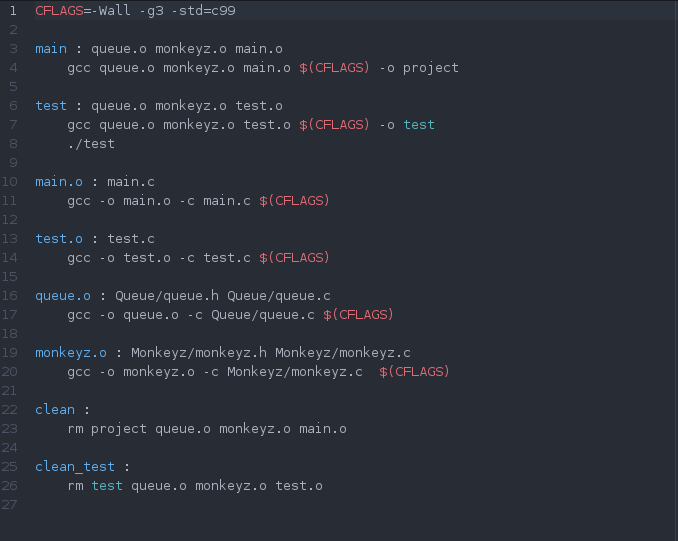
\includegraphics[width=\linewidth]{makefilebase.png}
    \caption{Makefile, version de base}
    \label{fig:makefilebase}
\end{figure}

Dans la figure \ref{fig:makefilebase}, nous pouvons voir que notre Makefile contient trois règles générales : 
\begin{itemize}
    \item une règle main, permettant de compiler le projet
    \item une règle test, permettant de compiler le fichier test.c et de lancer des tests unitaires
    \item une règle clean, qui permet de nettoyer le projet de tous les fichiers crées par la compilation des deux premières règles.
\end{itemize}
Nous utilisons aussi une variable \verb'CFLAGS' qui contiens toutes les options que nous appliquons au compilateur. Ainsi, si nous souhaitons modifier la façon dont nos fichiers sont compilés par gcc, il suffit de modifier la variable, ce qui est beaucoup plus pratique que de modifier toutes les lignes où le compilateur est appelé.
Au fil des \emph{achievements}, ce Makefile n'a que très peu changé, et a toujours conservé sa logique initiale.

\subsection{Structure de file simplement chaînée}
La structure de données abstraite qui sert de base au sujet est la file, une structure FIFO dont l'implémentation était guidée pour être réalisée à l'aide d'un amas de cellules. Concrètement il nous était conseillé de réserver en amont une grande quantité de mémoire organisée sous forme d'un tableau de cellules. La fougue de notre jeunesse nous poussât à faire fi de ces sages recommandations, et nous implémentâmes donc la file à l'aide d'une structure chaînée réservant et libérant la mémoire manuellement, cellule par cellule, à l'aides des fonctions \verb"malloc()" et \verb'free()'. Ce choix présentait l'avantage de nous permettre d'utiliser autant de mémoire que l'ordinateur peut en accorder sans se confiner à une quantité prédéfinie qu'on laisse en plus majoritairement vide la plupart du temps (quel gaspillage !).\\\\
\textbf{Important :} Ce choix de structure, que nous avons fait dès le départ, nous a empêché d'effectuer l'\emph{achievement} 5, qui repose sur l'idée que nous disposons d'un amas de mémoire. Nous ne pouvons pas recycler des cellules quand elles sont toutes tout le temps actives, et donc qu'aucune cellule n'est gaspillée en premier lieu.\\\\
Une file est donc composée d'un ensemble de cellules, chacune étant une structure contenant une chaîne de caractères, un entier, et un pointeur sur une cellule. La chaîne de caractère sert de support pour stocker des mots, une unité de base cohérente quand il est question d'écriture. L'entier remplit deux rôles distincts, qui seront abordés en même temps que les singes. Le pointeur enfin sert à chaîner la structure : il contient l'adresse de la cellule suivante dans la file si cette dernière existe, ce qui est indispensable pour parcourir ladite file.\\\\
Les cellules étant chaînées entre elles, il suffit pour implémenter la file d'enregistrer dans une structure dédiée un pointeur vers la première et un pointeur vers la dernière cellule de la file. Puisque chaque cellule pointe vers la suivante, cela permet de caractériser entièrement la file. On remarquera que la file ainsi créée n'est pas indexée.\\

L'ajout d'un pointeur sur le dernier élément permet d'ajouter une cellule dans la file en temps constant, car il n'est dès lors plus besoin de parcourir la file pour trouver l'emplacement du dernier élément.\\
Dans la version de base, deux files entrent en jeu : la file principale, utilisée par le singe lecteur et le singe imprimeur, et la file des statistiques, utilisée par le statisticien.%je sais pas où on met ça mais faut le mettre quelque part
\newpage
\subsubsection{Fonctions de la file}%on mettrait pas des sous-sous-sections avec le nom des fonctions ? ou même leur but (enfiler, défiler, etc) % non, car comme je le dit, les fonctions sont trop classiques pour s'y attarder
La file est une structure abstraite classique pour laquelle il faut implémenter des fonctions de base déterminées sur lesquelles nous allons donc passer rapidement.\\

\textbf{init\_queue : }initialise les pointeurs de la file à \verb'NULL', en faisant une file vide. Sa complexité est constante, car elle ne fait qu'un nombre fini d'initialisations de pointeurs, qui sont des opérations élémentaires. Elle doit être appelée sur toute file avant toute utilisation de celle-ci.\\

\textbf{add\_in\_queue : }enfile une cellule déjà créée dans une file. Pour des raisons de gestion mémoire, la cellule ajoutée doit être déclarée au préalable avec un \verb"malloc()". Elle initialise aussi la cellule ajoutée, nous évitant une fonction \verb'init_cell()'.\\

\textbf{pop\_queue : }après s'être assuré que la file n'est pas vide, supprime son dernier élément et en renvoie une copie. Dans le cas où la queue est vide, renvoie \verb'NULL'.\\
Cette fonction a une complexité temporelle constante.\\

\textbf{purge\_queue : }détruis toutes les cellules d'une file et libère l'espace mémoire réservé. Elle est appelée nécessairement à la fin du programme principal et ce pour toutes les files afin d'éviter une fuite mémoire.\\

Les fonctions qui suivent sont des fonctions de débogage (\verb print_queue()  par exemple), qu'il n'est pas utile de décrire.

\subsection{Conception des singes}
Les singes ont été implémentés à l'aide d'une structure de données qui contient, dans la version de base, quatre éléments. Le premier sert à réguler l'activité du singe en lui permettant de se mettre en grève quand ses revendications de travail ne sont pas remplies, le second à aliéner chaque singe de son individualité en l'associant tout entier à son activité professionnelle, et les deux derniers sont des compteurs qui permettent de contrôler leur productivité.
\begin{verbatim}
enum WORK_S { READER, STATISTICIAN, PRINTER };
struct monkey {
    int status ;           //boolean, equals 0 if on strike, 1 if active
    enum WORK_S work;      //his activity/role
    int read_words;
    int printed_words;
};
\end{verbatim}
\newpage
Les singes sont stockés dans un tableau de singes sobrement appelé \verb'monkeyz' où ils attendent patiemment d'être aléatoirement choisis pour participer à l'oeuvre commune. Quand viens leur tour de travailler, la fonction de travail principale \verb'work()' les redirige en fonction de leur activité vers des fonctions de travail secondaires propres à chaque activité.
Il va de soi que chaque singe a ses petits caprices et n'est donc pas enclin à travailler à tout instant. Quand il n'en a pas envie, il se met en grève. %Son envie est conditionnée par son activité aliénée.
La mise en grève des singes est gérée par une fonction indépendante \verb'filter_active_monkeys()' qui sera rapidement abordée dans la sous-section dédiée au travail.
%tu en étais là, j'ai rajouté des explications après. je pense que ce qui les intéresse le plus, c'est le j'ai fait comme ça, et "pourquoi t'as fait comme ça ?". Penser à mettre des schémas (jpense c'est mieux des schemas mais faut pas oublier de mettre un peu de code aussi jpense) pour illustrer ou de petits bouts de code. Là ça serait bien du coup d'expliquer work avec un schéma ou du code et de décrire les fonctions de travail des singes

%Nous avons en effet décidé dés le début de créer des fonctions complétement différentes pour chaque singe, afin de rendre le code plus clair. On avait donc, pour la version de base, trois fonctions, pour trois travails : \verb reader_work() , \verb printer_work()  et \verb statistician_work() . Ce que \verb work()  effectue est un simple test sur le travail du singe, qui lui permet de savoir vers quel fonction rediriger celui-ci. Concrètement, il s'agit d'un switch case.\\    Tu répètes juste +/- ce que je dis juste avant
%\\Image de l'algo de Work / ou schéma
%Nous avons aussi pris la décision de mettre les singe dans un tableau de données dès le début, afin de faciliter le processus de selection des singes actifs. De la même façon, cela nous permettait aussi de determiner quel singe était en grève en les mettant à la fin du tableau. (C'est ce qu'effectue la fonction \verb filter_active_monkeys()  ). ça c'est juste faux / bah non, c'est aussi pour les selectionner qu'on les a mit dans un tableau !!/Oui, mais on déplace pas leurs indices ou quoi et surtout pas dans filter_active_monkeyz / ah merde je croyais / c'est select_random qui fait ça en créant un nouveau tableau
\subsubsection{Le lecteur}
Le premier singe à considérer est le lecteur. Quand il est appelé, son travail consiste à détecter un mot, l'inscrire dans une cellule et ajouter cette cellule à la file de lecture.\\\\
Les principales difficultés auxquelles ce singe doit faire face sont la délimitation d'un mot et la détection de la fin du fichier, y compris quand ce dernier finit par des espaces, saut de lignes ou autres coquetteries inattendues. Pour ce faire il parcours simplement le fichier un caractère à la fois jusqu'à en trouver un qui ne puisse pas faire partie d'un mot, par exemple un espace, une tabulation ou la fin du fichier. Si il était jusqu'alors dans un mot, il le considère fini. Il est à noter que nous avons choisi, suivant les conventions du sujet, de considérer les groupements de mots séparés par des apostrophes tels que \emph{don't} ou séparés par un tiret tels que \emph{self-substantial} comme un mot unique, afin d'éviter des groupements séparés de lettres correspondant à des mots contractés qui n'ont aucun sens considérés seuls. Cela nous permet aussi d'être en cohérence avec les tests imposés en terme de nombre de mots lus.\\
Simple dans ses besoins, ce singe se met en grève lorsque la fin du fichier a été atteinte et qu'il ne reste aucun mot à lire.\\
Son travail concret se divise donc en deux étapes principales :
\begin{itemize}
    \item lire un mot du fichier et l'enregistrer dans une chaîne de caractères, ce qu'il fait en parcourant une seule fois le mot, caractère par caractère. Cette étape a donc une complexité linéaire en la taille du mot.
    \item placer cette chaîne de caractères dans une cellule et l'insérer dans la file. Cela se fait au prix de deux parcours du mot, un pour le formater en terme de casse, un autre pour le copier dans une cellule nouvellement créée. La création de la cellule et son ajout dans la queue se font tous deux en temps constant, ce qui laisse cette étape avec une complexité linéaire en la taille du mot également.
\end{itemize}
Une dernière tâche mineure est d'incrémenter son compteur du nombre de mots lus, ie son attribut \verb:read_word:.

\subsubsection{Le statisticien}
La tâche du statisticien est relativement simple. Il examine la dernière cellule de la file principale, puis l'ajoute dans la file statistique si c'est un mot qu'il n'a jamais vu, ou incrémente la multiplicité du mot dans la file statistique si il l'a déjà vu.\\
Cela nous amène au double usage de l'attribut \verb was_read_by_statistician  des cellules : dans la file principale, il sert de booléen pour que le statisticien puisse savoir si oui ou non il a déjà lu le dernier mot de la file ; dans la file statistique il sert à compter la multiplicité d'apparition des mots. Si il a effectivement déjà lu le dernier mot de la file principale, il se met en grève.\\
La principale opération réalisée par ce singe est la copie d'une cellule, qui se fait en temps linéaire de la longueur du mot qu'elle contient.\\

\subsubsection{L'imprimeur}
L'imprimeur a le rôle de nettoyeur de la file principale, il défile les cellules générées par le lecteur et imprime le mot qu'elles contiennent sur la sortie standard. Il se met en grève quand le statisticien n'a pas encore vu le dernier mot de la file, pour éviter que certain mots ne soient pas traités. Il compte également le nombre de mots qu'il a imprimés. Il réalise tout cela en complexité constante.\\

\subsection{Implémentation de l'algorithme principal}
L'algorithme principal se situe dans le fichier main.c. Nous n'avons rien vraiment crée car il nous a été fortement inspiré par celui présent sur l'énoncé de départ.\\
C'est cet algorithme qui est représenté dans notre code :
\begin{verbatim}
  84     filter_active_monkeys(monkeyz, NB_OF_MONKEYZ, main_queue, read_file);
  85     while(!all_on_strike(monkeyz)){
  86         struct monkey* happy_selected_monkey = random_select(monkeyz, [...]);
  87         work(happy_selected_monkey, &main_queue, &stats_queue, read_file);
  88         filter_active_monkeys(monkeyz, NB_OF_MONKEYZ, main_queue, read_file);
  89     }
\end{verbatim}

\subsubsection{La fonction filter\_active\_monkeys}
La fonction \verb filter_active_monkeys  parcours le tableau \verb monkeyz[]  et effectue un test en fonction du travail du singe testé pour déterminer si oui ou non il décide de se mettre en grêve.\\
Le programme ne s'arrête que quand les singes ne peuvent plus travailler, au moins dans la version de base. \verb'filter_active_monkeys' admet une complexité linéaire en la taille du tableau des singes.\\

\section{Développement de l'\emph{achievement} 1}
\subsection{Énoncé de la problématique}
Les singes sont finalement parvenus non sans mal à utiliser une file fonctionnelle pour s'échanger des données, et à s'organiser dans leur travail pour produire du texte en anglais. Cependant, il y a un bémol ! Les singes ne \emph{produisent} pas du texte, ils ne font que recopier le contenu du fichier que nous leur donnons en paramètres.\\
Là est la problématique principale de cet \emph{achievement} : il s'agit de créer un nouveau singe, l'écrivain, capable de créer du texte à l'aide des mots que son collègue \emph{le lecteur} lirait. Le comportement de l'écrivain est imposé :
\begin{itemize}
    \item pour commencer à écrire il doit tirer aléatoirement un mot dans la file du statisticien, qu'il garde en mémoire
    \item il regarde alors parmi les successeurs de ce mot, et en prend un au hasard, qu'il ajoute à sa phrase, et qui devient le nouveau mot mémorisé
    \item si le mot qu'il avait choisi ne possède aucun successeur, ou sur une chance de 0,1, il termine sa phrase
    \item pour ce faire il génère une ponctuation aléatoire si la phrase contient plusieurs mots, un point d'exclamation si elle n'en contient qu'un seul, et retourne à la première étape
\end{itemize}
Ce changement apporte son lot de nouvelles problématiques à régler. La plus grande est le calcul des successeurs. En effet, le statisticien doit maintenant pouvoir enregistrer les successeurs de chaque mot. Nous verrons dans la suite de ce document que cela nous à nécessité la création d'une nouvelle structure de données, exclusif au statisticien : la \emph{file de successeur}.\\
\subsection{Modification du statisticien}
\subsubsection{Conception de la file des successeurs}
Pour permettre au statisticien de mémoriser les successeurs de chaque mot lu, nous avons décidé de lui créer une nouvelle structure de données exclusive. L'idée est simple : puisque que le singe imprimeur prend désormais ses données de la file de l'écrivain et non plus du lecteur, il incombe au statisticien de lire et vider la file du lecteur et d'enregistrer les mots ainsi lu dans une nouvelle file. Cependant une file classique comme celle que nous utilisions jusqu'ici ne permettait pas de décrire ce concept de successeurs. Plutôt que de modifier grandement la structure déjà existante, nous en avons développé une nouvelle.
Dans cette nouvelle structure, qui est aussi une file au sens général du terme, et que nous désignerons par le nom de file de successeurs, chaque cellule contient en plus des éléments intrinsèques à la file de base, un pointeur vers une file classique qui servira à stocker les successeurs du mot de la cellule et leur multiplicité d'apparition.
\subsubsection{Le calcul des successeurs}
Une fois cette structure de données pensée et implémentée, il s'agit de la remplir. Cela est du ressort du statisticien. Du fait de la séparation des files, il n'a maintenant plus besoin de savoir si il a lu le dernier mot de la file du lecteur, mais doit en revanche le défiler. Ce n'est évidemment pas le changement le plus dur à implémenter. Cependant cela veut dire qu'au moment de placer le mot dans la file des successeurs d'un autre mot, la cellule contenant le mot précédent dans la phrase a déjà été supprimée.\\
Le calcul des successeurs se fait donc de la manière suivante : quand le statisticien voit un mot, il le copie dans une cellule volante, non rattachée à une file. Ainsi quand il lit le mot suivant, il peut librement le placer non seulement dans la file des statistiques principales, mais aussi identifier son prédécesseur et l'ajouter dans la file des successeurs dudit prédécesseur, ou augmenter sa multiplicité dans cette file.\\
\subsection{Développement du singe écrivain}
Ce qui nous a posé le plus de problèmes avec l'écrivain n'était pas sa conception de base (à savoir créer des mots à partir des anciens). Nous avions déjà l'idée en tête : il fallait juste prendre des cellules au hasard dans la file du statisticien, l'ajouter dans une file dédié à l'écrivain, répéter ça à chaque fois et le travail était fini.\\ 
Nous n'avions alors pas pensé à la structuration d'une phrase ! Comprenez par là : arrêt d'une phrase avec un point d'exclamation si elle ne possède qu'un mot, utilisation d'un mot de ponctuation aléatoire pour finir sa phrase, etc... Pire, dans notre mauvaise compréhension du sujet, nous avions fait fi d'une partie du travail de l'écrivain : il ne souvenait donc pas du mot qu'il avait pris au dernier tour où il travaillait, et prenait parmi les successeurs d'un nouveau mot aléatoire chaque tour. Ce qui, au final, enlève tout ce qu'était censé apporter cette contrainte de l'énoncé : une sorte de cohérence (toute relative) dans les phrases de l'écrivain.\\
Nous retrouvant avec ce singe écrivain à moitié fou, nous avons donc étudié nos possibilités. Le plus important était de permettre au singe écrivain de se rappeler du dernier mot qu'il avait écrit afin de faire une phrase cohérente. \\\\
Pour ce faire, notre solution était simple : il suffisait de donner au singe écrivain un accès à une chaîne de caractère, dans laquelle il stockerait le dernier mot qu'il avait mémorisé. Cette chaîne a été appelée \verb memorized_word[] . Cependant, dans notre précipitation, nous avons fait une petite erreur de conception : nous le lui avons passé en paramètre de sa fonction, ce qui alourdissait le nombre de paramètres nécessaire au travail de l'écrivain, et donc, de ce fait, le nombre de paramètres nécessaire à la fonction générale de répartition du travail \verb work() .\\Nous aurions pu, pour simplifier la chose, najouter \verb memorized_word[]  directement dans la structure des singes.\\\\
Pour connaître la longueur d'une phrase nous avons opéré de la même façon : en lui donnant accés à un entier, \verb writer_sentence_length , qui contient donc la longueur de la phrase qu'il est actuellement en train d'écrire.\\\\
Ces soucis de conception ont cependant été corrigés à l'\emph{achievement} 2, lorsque nous avons dû mettre en place des pointeurs de fonctions.\\
\subsubsection{Complexité du singe écrivain}
Les sous-fonctions qu'utilisent notre singe écrivain dans sa fonction \verb writer_work()  ne sont que des fonctions de recherche et de sélection aléatoire dans la file. Les fonctions de recherches sont linéaires, car nous parcourrons toute la file. La fonction de sélection aléatoire aussi. Le traitement qu'effectue notre preux singe n'ajoute que peu de complexité de temps à cela (ce ne sont que des instructions impératives sans boucles, donc en temps constant). L'écrivain travaille donc en temps linéaire.\\
Nous ne savions pas trop comment procéder autrement, car pour rechercher un mot dans la file, il faut nécessairement parcourir toute la file. Si elle était triée par ordre alphabétique, nous aurions pu tenter une approche dichotomique (en \emph{logn}), mais cela aurait eu pour coût de devoir trier le tableau à chaque ajout de cellule, nous empêchant donc de faire des ajouts en temps constant. Nous avons donc préféré ne rien changer.

\section{Développement de l'\emph{achievement} 2}
\subsection{Enoncé de la problématique}
L'idée de cet \emph{achievement} est d'ajouter à notre système de singe un nouveau singe lecteur, travaillant en parallèle de l'ancien et lisant un autre fichier (ou le même), et un nouveau singe écrivain, travaillant lui aussi en parallèle de l'ancien.\\
Pour réaliser cet \emph{achievement}, chaque singe lecteur doit donc avoir sa propre file, sur laquelle il enregistre les mots qu'il lit, et son propre ficher. Le statisticien, lui, communiquerait avec les deux écrivains (donc avec leur deux files). Puis arrivent les deux écrivains, qui donc communiquent tous les deux avec la file du statisticien. En bout de chaîne se trouve l'imprimeur, qui imprime les phrases des deux écrivains en même temps.\\
De façon imagée, cela nous donne un schéma du type de la figure \ref{fig:explicationachievement2}.

Autre fonctionnalité demandé : les singes doivent maintenant avoir accès à leur fonction de travail personnelle par le biais d'un pointeur de fonction directement intégré à leur structure. Ce changement d'organisation invalide donc notre ancienne fonction \verb work()  .

\begin{figure}[h]
    \centering
    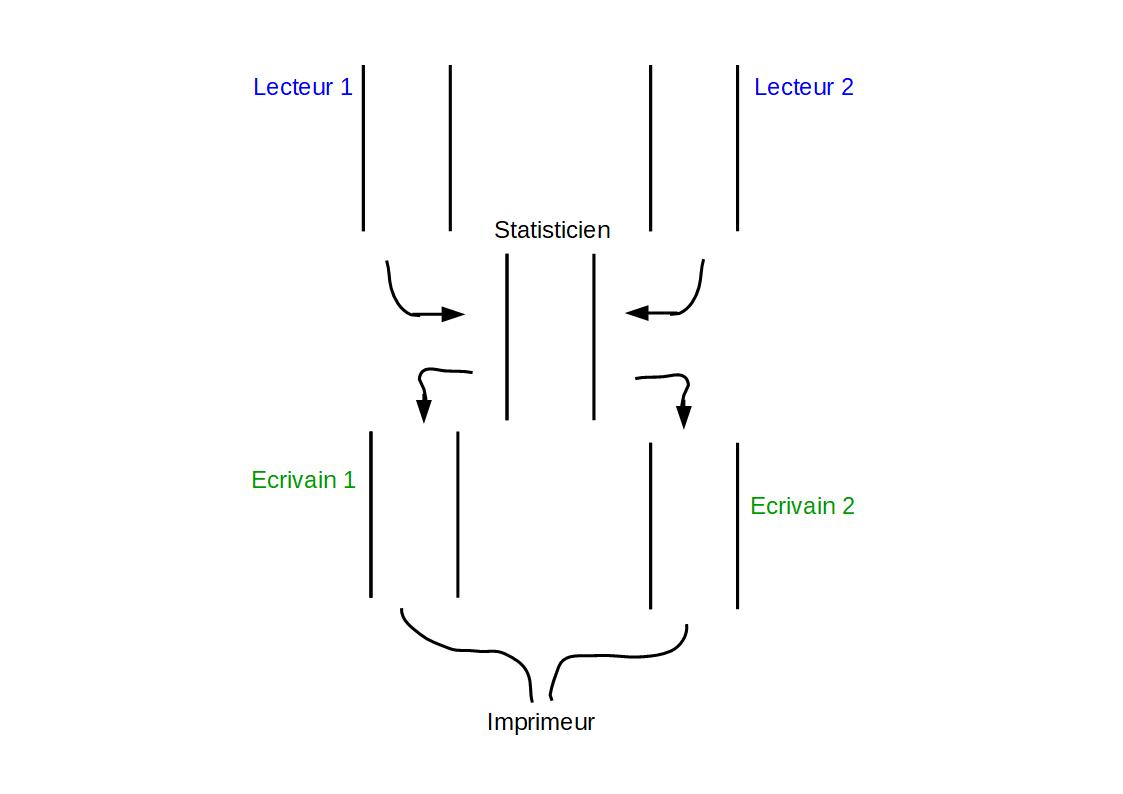
\includegraphics[width=\linewidth]{yo.jpg}
    \caption{Illustration du fonctionnement demandé pour l'Achievement 2}
    \label{fig:explicationachievement2}
\end{figure}


\subsection{L'ajout des singes}
Pour créer ces singes, nous avons choisis d'ajouter dans l'énumération \verb WORK_S  un nouveau reader ainsi qu'un nouveau writer, ce qui nous donne une énumération de ce type : 
\begin{verbatim}
    enum WORK_S { READER_1, READER_2, [...], WRITER_1, WRITER_2 }
\end{verbatim}
Ceci fait, il nous est possible d'une façon très simple de tester quel singe est en train de travailler : il suffit de tester son \verb WORK_S .
Maintenant, la problématique est la suivante : comment faire pour savoir dans quelle file doit écrire tel singe lecteur ? Comment savoir dans quel fichier lire ? Nous pourrions passer en paramètre de la fonction globale \verb Work()  toutes les file et tous les pointeurs \verb FILE* ,  pour ensuite faire le tri dans la fonction \verb reader_work()  , mais cela n'est pas très propre, peu modulable et lourd à implémenter. Si l'on nous demandait d'ajouter encore des singes, il faudrait redoubler le nombre de paramètres en conséquence. Cette solution n'est donc pas souhaitable.
Nous avons alors pris la décision de modifier directement la structure des singes, afin de leur implémenter une file personnelle, ainsi qu'un pointeur \verb FILE*  . Cela peut aussi avoir ses défauts, et l'on pourrait nous reprocher de rajouter des données qui seraient inutiles pour les autres singes, mais c'était à nos yeux plus simple et plus correct que d'appliquer l'autre solution.\\
\subsubsection{Le nouveau calcul des successeurs}
L'ajout d'un nouveau singe lecteur amène un tout nouveau problème : l'implantation que nous avions validé pour l'\emph{achievement} 1 n'est plus valide. En effet, dans l'\emph{achievement} 1, c'était le statisticien qui mémorisait le dernier mot qu'il avait lu dans la file du lecteur. Cependant, il ne peux plus agir ainsi : Il risquerait de confondre les deux fichiers, et donc de créer des successeurs inexacts !
Nous avons donc dû changer la réalisation du calcul des successeurs.\\
Pour cela, nous avons eu une nouvelle idée. Plutôt que le statisticien se rappelle du dernier mot qu'il a traité, il n'aurait qu'a regarder le prochain mot disponible dans la file du lecteur dont il s'occupe ! Ainsi, plus de problèmes de successeurs inexacts, vu qu'il prendrait le successeur directement à la source du lecteur concerné. \\ 
Cependant, cette solution arrive avec un nouveau problème. \textbf{Si la file du lecteur ne comporte qu'un mot, il est alors impossible de connaître son successeur via cette méthode}. Heureusement, il existe une solution : Nous avons modifié le comportement du singe lecteur pour qu'il puisse lire les mots \textbf{deux par deux, et qu'il conserve toujours au moins deux mots dans sa file} attitrée, sauf quand il arrive à la fin du fichier (Comme il s'agit du dernier mot, il n'a logiquement pas de successeur).
Cela nous amène donc aussi à modifier les conditions de grève des singes : le statisticien doit se mettre à travailler si et seulement si il y a au moins deux mots dans une des files des lecteurs (sauf si les lecteurs sont arrivés à la fin de leur fichier). De même pour le lecteur, si il y a deux mots dans sa file (ou si il est parvenu à la fin de son fichier) s'en ira mener la lutte. C'est ce nouveau comportement qui est décrit dans la figure \ref{fig:schema_reader_new_attitude}.

\begin{figure}[H]
    \centering
    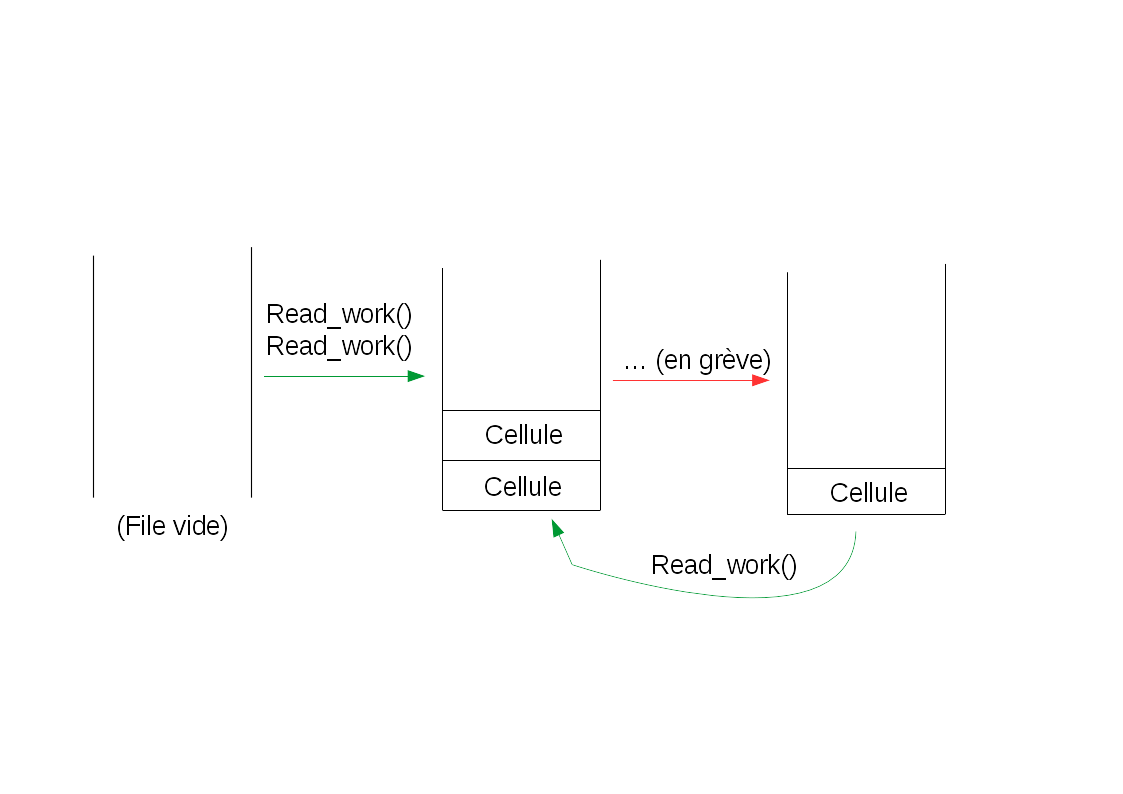
\includegraphics[width=\linewidth]{rapport_schema_1.png}
    \caption{Schéma du nouveau fonctionnement du singe lecteur}
    \label{fig:schema_reader_new_attitude}
\end{figure}

\subsubsection{L'ajout du nouveau singe écrivain}
Comme indiqué dans l'énoncé, il fallait que l'imprimeur ait une nouvelle condition de grève (ou plutôt, de non grève). En effet, les écrivains devaient désormais se mettre en grève dès qu'ils avaient terminé une phrase, puis attendre que le singe imprimeur vide leur file. En suivant cette logique, le singe imprimeur ne devait travailler que si un des écrivains avait terminé une phrase. Nous avons donc décidé d'utiliser un drapeau, un booléen signalant qu'un des écrivains était arrivé à la fin de sa phrase.
Nous étions alors confronté à la même problématique qu'au début de cet \emph{achievement} : Fallait-il passer en paramètre ce flag, pour chacun des deux singes, et au singe imprimeur ? Ou l'implémenter directement dans la structure du singe ?
Finalement, nous avons encore opté pour la seconde solution, qui est à nos yeux la meilleure façon de résoudre ce problème. Une autre solution aurait été de ne pas choisir d'utiliser un flag, mais de regarder directement sur la file des écrivains si leur dernier mot enregistré était un signe de ponctuation. Mais l'option choisie semblait plus simple à comprendre et implémenter, c'est pourquoi nous nous y sommes accrochés.\\
C'est ainsi que nos singes accueillèrent un nouvel entier, faisant office de drapeau : \verb sentence_finished  .
\subsection{Implémentation du pointeur de fonction}
Lors de l'ajout du pointeur de fonction dans la structure des singes, nous avons été surpris par une difficulté que nous n'avions pas imaginée. Pour créer un pointeur de fonction, il faut nécessairement que le pointeur ait la même signature que la fonction sur laquelle il pointe. Or, nos différentes fonctions de travail  avaient des signatures  très différentes. Ici, deux solutions se proposaient à nous : 
\begin{itemize}
    \item Créer un pointeur pour chaque fonction de travail dans la structure des singes
    \item Réduire le nombre de paramètres de chaque fonction de travail pour les uniformiser
\end{itemize}
Nous avons préféré la seconde solution car elle offrait plus de modularité au code. Cela serait en effet plutôt lourd et long d'ajouter un nouveau pointeur de travail spécifique dans la structure globale des singes si nous étions amenés un jour, par exemple, à en créer d'autres, alors qu'il suffit à la création d'une fonction de se restreindre à un certains nombres d'arguments.\\
Oui, mais alors dans ce cas, comment garantir que le nombre d'arguments sera toujours satisfaisant ? \\
Et bien dans les faits, nous ne le pouvons pas. Cependant, cela ne signifie pas que nous pouvons prévenir ce problème d'arriver un jour ! C'est pour quoi nous avons décidé de garder en paramètre :
\begin{itemize}
    \item Le singe qui effectue le travail
    \item La file du statisticien
    \item le tableau général des singes
\end{itemize}
Cela permet déjà beaucoup d'autres applications que nous en avons dans notre programme. Avec le tableau des singes, chaque singe peut littéralement accéder à n'importe quelle ressource de ses collègues, et ce facilement qui plus est car il est possible d'utiliser l'énumération \verb WORK_S  afin de se déplacer dans le tableau. (Tout cela est rendu possible car le tableau des singes \verb monkeyz[]  est indexé par cette énumération).\\\\
Le seul paramètre qui peut sembler superflu ici est la file du statisticien, que nous avons laissé par obligation, car c'est le seul singe à ne pas avoir sa file directement intégré dans sa structure (hors l'imprimeur qui n'a pas besoin de file) et donc à la nécessiter dans ses paramètres.\\
En effet, nous avons rajouté une file normale dans la structure des singes, et pas une \emph{file de successeur}. La file des successeurs étant plutôt unique en son genre, nous avons pensé qu'il serait inutile, voire même superflu d'ajouter ce type de file dans la structure globale des primates sachant que probablement, le statisticien sera le seul singe à avoir besoin de ce genre spécial de liste chaînée dans le futur.

\section{Fonctions de Tests}
Pour assurer que notre programme fonctionne bien sur toute la ligne, nous avons crée quelques fonctions tests permettant de tester de façon indépendante les fonctions. (C'est à dire qu'on effectue des tests unitaires : Une fonction à la fois).\\
Lors de notre développement, nous n'avons pas conservé nos tests, les réalisant à la volée. De plus nous avons vite commencé à utiliser des programmes comme gdb ou valgrind pour débugger. Cependant, cela ne signifie pas que nous n'avons à l'heure d'aujourd'hui aucun tests, car quelques fonctions de testing ont été codées après que l'\emph{achievement} 2 ait été réalisé. D'une part car il est toujours utile d'en avoir, et d'autre part car le fait que l'\emph{achievement} 2 marche pour l'instant ne garantit pas que notre programme est sans faille. 
\subsection{Stress Test de la file}
Ce stress test crée successivement beaucoup de cellules dans plusieurs files, et vérifie que la file à autant de cellules qu'elle devrait en contenir, ni plus, ni moins. Ce test permet notamment de voir si la file n'a aucun bug sur la création et le chaînage de cellules, et teste par la même occasion la fonction \verb length_queue() , fonction renvoyant le nombre de cellules d'une file.
\subsection{Tests unitaires des fonctions}
Nous avons ensuite essays de réaliser le plus de tests unitaires possibles sur les fonctions de nos fichiers \emph{.c}.
Nos tests s'appliquent fonction par fonction, et toujours de la même manière : Nous créons un cadre favorable au lancement de la fonction, puis nous effectuons successivement des \verb assert()  permettant de tester si l'état des données après le passage de la fonction est cohérent tout en modifiant le cadre dans laquelle la fonction s'effectue.\\
Ainsi, si à un moment, l'état des données n'est pas conforme à nos attentes, \verb assert()  termine le programme en indiquant quel test à échoué. Si tout se passe bien, \verb assert()  ne fait rien et le test passe donc sans encombres. C'est ce comportement qui est montré dans le code verbatim suivant :

\begin{verbatim}
void pop_queue_test(struct queue* queue)
{
    printf("Testing pop queue...\n");

    struct cell* cellb = malloc(sizeof(struct cell)); //Création de l'environnement
    struct cell* cella = malloc(sizeof(struct cell)); //propice au lancement...
    strcpy(cella->word,"A");
    strcpy(cellb->word,"B");
    add_in_queue(cella,queue);
    add_in_queue(cellb,queue);

    struct cell popped = pop_queue(queue);

    assert(strcmp(popped.word,"A") == 0); //Tests de la cohérence des données...
    assert(strcmp(queue->first->word,"B") == 0);

    printf(GRN "OK\n" RESET);
}
\end{verbatim}
A l'heure où ce rapport est écrit, seulement les fonctions de \verb queue.c , et quelques fonction de \verb monkeyz.c  sont testées. Par manque de temps, nous n'avons pas pu réaliser plus de tests.

\section{Conclusion}
Ce projet a été l'occasion d'apprendre de notre binôme respectif des techniques de travail et de programmation dont nous n'avions pas forcément conscience en le démarrant. C'est même sans doute cette interaction qui nous a le plus appris pendant toutes ces semaines.\\
Notre développement n'a pas été parfait.
Nous avons commis quelques erreurs lors des conceptions, c'est-à-dire quand nous réfléchissions sur les solutions aux problématiques du projet. Nous étions trop pressés à coder, et nous avons au final perdu un peu de temps en n'en prenant pas assez à réfléchir. \\
D'un autre côté, nous avons aussi réussi à corriger au fur et à mesure notre code pour construire dessus une version fonctionnelle pour chaque \emph{achievement} avec des temps de débuggage plus limités que d'autres camarades.\\
Une autre source de problèmes a été l'utilisation de Git, outil dont notre maîtrise a tous les deux était très limitée et qui, malgré l'aide de nos encadrants, nous a mené à quelques quasi-catastrophes et des pertes de temps énormes.
En résumé, cela nous a permis de mettre en application de bonnes méthodes de programmation, mais aussi d'expérimenter pourquoi elles étaient meilleurs dans des conditions plus proches du réel qu'un TD.\\

En ce qui concerne notre programme final, il est encore améliorable, en ce sens que beaucoup de fonctions que nous avons écrites peuvent être optimisées en nombre d'instructions, en clarté, en modularité. Malgré tout, nous avons essayé de factoriser notre code au maximum, afin que dans tous les cas, la maintenabilité de notre programme soit assurée, permettant ainsi, dans le futur, que d'autres singes fougueux et ambitieux puissent eux aussi s'essayer à écrire du Shakespeare.\\
 C'est donc instruit que nous ressortons de ce premier projet en binôme, prêt à faire face à de nouvelles problématiques lors des prochains projets. Tout ce que nous espérons, c'est que des singes soient encore de la partie.


\end{document}
